One can also model the van Keken problem with the volume-of-fluid (VOF) interface tracking 
algorithm in \aspect{}.
In fact, this problem is particularly well-suited to being computed with the VOF method, since 
it consists of two distinct, immiscible fluids and interface tracking algorithms are 
specifically designed not to allow the two fluids to mix.
In particular, assuming the computation is sufficiently well-resolved, the fluids will not mix 
at sub-grid scales over the entire duration of the computation.
However, note that this implies that all computations of the van Keken problem made with the VOF 
method must necessarily be with discontinuous initial conditions.
Finally, since one is often interested in a high resolution image of the shape of the interface 
between the two fluids, one can use the output of the VOF method to examine the interface 
within individual cells or within regions consisting of groups of cells.

Another advantage the VOF method has over modeling moving interface problems with compositional 
fields is that for problems in which the interface occupies a relatively small part of the 
computational domain, all of the computational work in the VOF method is done in cells that lie 
in a neighborhood of the interface, rather than in the entire computational domain. 

\begin{figure}
   \centering
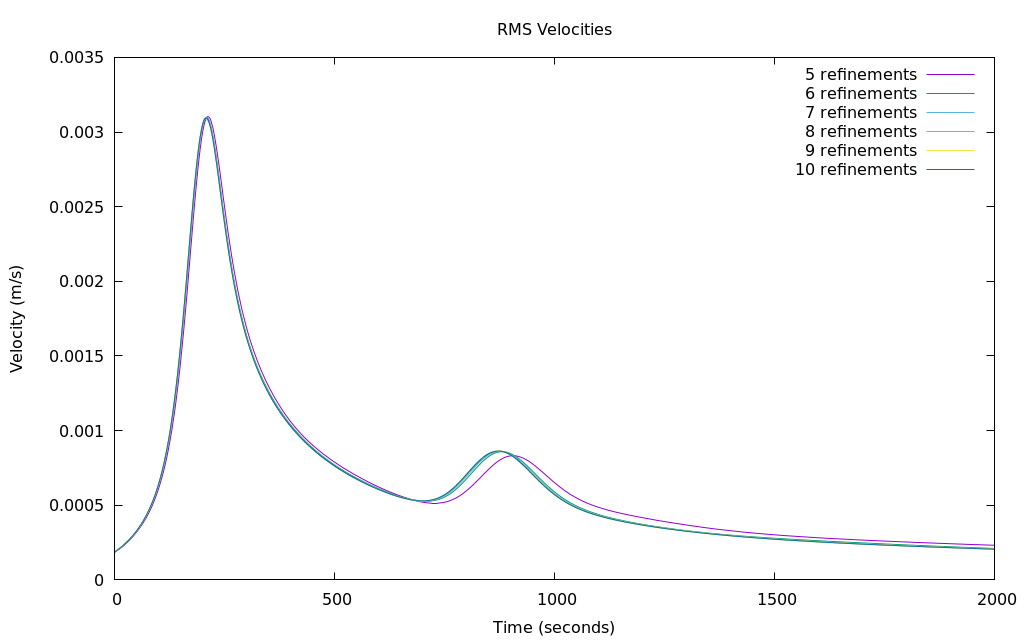
\includegraphics[width=0.5\textwidth]{cookbooks/van-keken-vof/doc/rms_vel_comparison.png}
   \caption{Evolution of the root mean square velocity as a function of time for computations 
    of the van Keken problem made with the VOF interface tracking algorithm with five 
    different global mesh refinements.
    Since the VOF initial conditions are discontinuous, the above results should really be 
    compared with the computations with discontinuous initial conditions on the left in 
    Figure~\ref{fig:vk-2}. However, the above results also compare extremely favorably with the 
    computations with smoothed, continuous initial conditions for the compositional field on 
    the right in Figure~\ref{fig:vk-2}.
    As in Figure~\ref{fig:vk-2}, 5 global refinements correspond to a $32 \times 32$ mesh and 10 global refinements correspond to a $1024 \times 1024$ mesh.}
    \label{fig:vof-vk-1}
\end{figure}

\begin{figure}
    \centering
    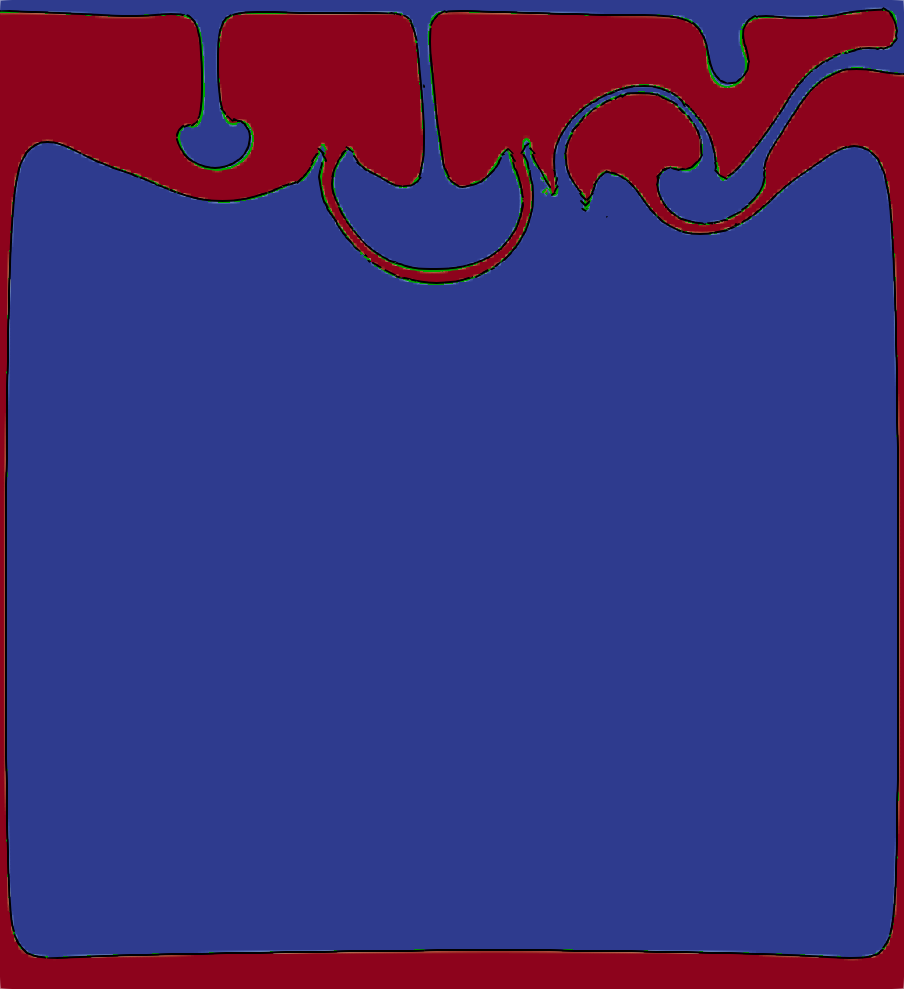
\includegraphics[width=0.4\textwidth]{cookbooks/van-keken-vof/doc/vof_van_keken_refinement_comparison.png}
    \caption{\it The results of two computations of the van Keken problem made with the VOF 
        interface tracking algorithm overlaid upon each other at $t_\text{end}=2000$.
        This visualization shows the reconstructed boundary between the two
        materials at the final time $t_\text{end}$ as computed on a uniform grid
        with 7 and 8 levels of refinement.
        The boundaries between the materials are displayed as contours
        of the fields $\tilde{\psi}^7(t_\text{end})$ (black) and
        $\tilde{\psi}^8\,(t_\text{end})$ (bright green), which are generated by the  visualization postprocessor.
        The contours for the reconstructed material boundaries are superimposed
        on a color gradient visualization of the material composition for the
        computation with 8 levels of refinement in order to make the regions
        with each fluid type more evident.
        Compare with the fourth image on the right in Figure~\ref{fig:vk-1}.
    }
    \label{fig:VOF_van_Keken-02}
\end{figure}

Since, as noted above, when the interface is discontinuous, the van Keken problem is a version 
of the Rayleigh-Taylor problem, which is unstable to perturbations of all 
wavelengths\footnote{This is true whether the two fluids have the same viscosity or different 
viscosities.} (e.g. see~\cite{SC:1961}).
Therefore, it is extremely sensitive to the initial conditions.
In order to address this sensitivity, we do not use  the default approach of
computing the initial material volume fractions using a composition quadrature.
Instead we compute the initial volume fractions using a signed distance
function $\phi$ as follows~\cite{JMR:2019,JMR-EGP:2019}.

First we create the function $\phi$, which has the following two properties: 1) it is positive 
in the region that contains one of the fluids, which we will refer to as fluid~1, and negative 
in the complement of this region, which we will refer to as fluid~2, and 2) at each point in 
the domain the magnitude $| \phi |$ of $\phi$ is the distance to the boundary between the 
two fluids or materials.
In the computations shown here, we use an approximation $\tilde{\phi}$ to $\phi$ such that   
difference between $\tilde{\phi}$ and $\phi$ is small enough for the purposes of making the 
computations high-quality.
The primary advantage of choosing this particular initialization algorithm is that it allows us 
to more accurately reproduce the initial condition on a sub-grid scale than would otherwise be 
possible on the coarser grid on which we compute the time evolution of the interface. 


\lstinputlisting[language=prmfile]{cookbooks/van-keken-vof/doc/main.part.prm.out}

The relevant sections of the parameter file for this type of initialization of the VOF method 
appears immediately above.
In particular, the combination of \texttt{Number of initialization samples} with the 
\texttt{level set} initialization type indicates that our initialization will consist of 
dividing each grid cell into $16 \times 16$ subcells and the distance to the given initial 
interface $f(\mathbf x)$, provided in \texttt{Function expression}, is computed in each of the 256 
subcells.
We then use this information to compute a piecewise linear interface approximation to $f(\mathbf x)$.
The volume fraction in each subcell is then found in the manner described 
in~\cite{JMR:2019,JMR-EGP:2019}.
This initialization procedure provides a much finer and thus, more accurate, initial condition 
than the standard VOF initialization procedure described above.

While the visualization configuration in a typical parameter file is sufficient for most 
purposes, when using the VOF method one has the ability to see the division between the fluids 
reconstructed by the VOF algorithm in each cell.
This is accomplished by plotting the zero contour of a field $\tilde\psi$ that
is generated to be $0$ on the reconstructed interface, positive in the region
with fluid~1, and negative in the region with fluid~2.
However $\tilde{\psi}$ does not satisfy the requirement that the magnitude is
equal to the distance to the interface as would be required for the signed
distance function $\phi$.
The modifications to the parameter file that are necessary in order to draw the reconstructed 
boundary as a contour are shown immediately below.
The full configuration file for this version of the benchmark problem can be found at 
\url{cookbooks/van-keken-vof/van-keken-vof.prm}.

\lstinputlisting[language=prmfile]{cookbooks/van-keken-vof/doc/postprocess.part.prm.out}
\noindent

We made a number of computations of the van Keken problem with the VOF method in order to 
compare the wall clock times with computations using a DG compositional field.
We ran both on the same cluster at global refinements 5--8 using one node with four CPUs and 
refinements 9 and 10 using two nodes with 16 CPUs.
Our results are shown in Table~\ref{tab:vof-runtime-comparison-table}.
In all of the computations shown in Table~\ref{tab:vof-runtime-comparison-table} we used a CFL 
number of $\sigma=0.5$.
Due to the change in the CFL number from $\sigma = 1.0$ in Table~\ref{tab:runtime-table} to 
$\sigma = 0.5$ in Table~\ref{tab:vof-runtime-comparison-table} and the difference between HPC 
clusters on which the computational results shown in the two tables were made, we can't make a
direct quantitative comparison between the data in Tables~\ref{tab:runtime-table} 
and~\ref{tab:vof-runtime-comparison-table}.

However, we can compare the required run time for a VOF computation to that for a DG computation.
We note that the use of the VOF advection algorithm significantly reduces the
required computation time in all cases, frequently requiring less than half the
time required by the DG compositional field.

We now examine the RMS velocity data shown in Figure~\ref{fig:vof-vk-1}.
Other than for the case of 5 levels of uniform global refinement, the curves for the RMS 
velocities for $6$, $7$, $8$, $9$ and $10$ levels of refinement in Figure~\ref{fig:vof-vk-1} 
are nearly indistinguishable.

Upon examining the solution at the final time, we note that the general structure of the 
solution shown in Figure~\ref{fig:VOF_van_Keken-02} matches the form and the general structure 
found in other versions of this benchmark such as the fourth image on the right in 
Figure~\ref{fig:vk-1}.
We also note that the differences in the shape of the interface based on a single refinement 
as shown in Figure~\ref{fig:VOF_van_Keken-02} are minor, although still slightly visible.
This is to be expected as refinement is a perturbation of the initial condition at a smaller 
wave length.

\begin{table}
  \centering
   \begin{tabular}{|c|c|c|c|}
     \hline
      Global Refinement & Number of Processors & VOF & DG \\
      \hline
\phantom{1}5 & \phantom{1}4 &\phantom{6}1.33 minutes\phantom{hours} &\phantom{1}2.57 minutes  \\
\phantom{1}6 & \phantom{1}4 &\phantom{1}8.51 minutes\phantom{hours} & 19.5\phantom{7} minutes \\
\phantom{1}7 & \phantom{1}4 &\phantom{1}1.15 hours\phantom{minutes} & \phantom{1}2.49 hours\phantom{tes} \\
\phantom{1}8 & \phantom{1}4 &\phantom{1}8.53 hours\phantom{minutes} & 19.6 hours\phantom{tes} \\
\phantom{1}9 & 16           &         16.30 hours\phantom{minutes}  & \phantom{1}2.72 days\phantom{tes} \\
          10 & 16           & \phantom{1}5.17 days\phantom{minutess}&>6.00 days\phantom{tess} \\
            \hline
        \end{tabular}
        \caption{\it Comparison of runtimes for the van Keken problem with VOF
            and a DG compositional field, in which the initial conditions for
            DG smoothed are as described in section~\ref{paragraph:van-keken
            compositional fields} above.  The times shown are for the full
            computation, ending at $t_\text{end} = 2000$ with a CFL number of
            $\sigma=0.5$ in both cases. 
            All of these computations were made with ASPECT version 2.2.0-pre
            (master, commit \texttt{ef542ecc2}) in release mode on the Peloton2 cluster at
            U.C.~Davis.
            We note that the change in the CFL number $\sigma$ and the
            differing choice of cluster makes a direct quantitative comparison
            between this table and Table~\ref{tab:runtime-table} invalid due to
            too many confounding factors.
        }
        \label{tab:vof-runtime-comparison-table}
\end{table}

The consistency of the results shown here differs noticeably from the behavior of the  
problem with discontinuous initial conditions when computed with the FEM and DG advection 
algorithms.
One possible reason for these differences is the specialized initialization procedure used for 
the volume of fluid method, which permits a much more consistent initialization by 
reducing the variation in the initial condition when the initial mesh is refined.

To study this feature of our algorithm and the sensitivity of the problem to
the precise initial condition, we vary the size of the initial interface
perturbation and examine the sensitivity of the final results to a small change
in the initial conditions.
Specifically, we vary the amplitude $a$ of the cosine function in the initial conditions, as 
shown below.

\lstinputlisting[language=prmfile]{cookbooks/van-keken-vof/doc/variation.part.prm.out}

\begin{figure}[htb]
    \centering
    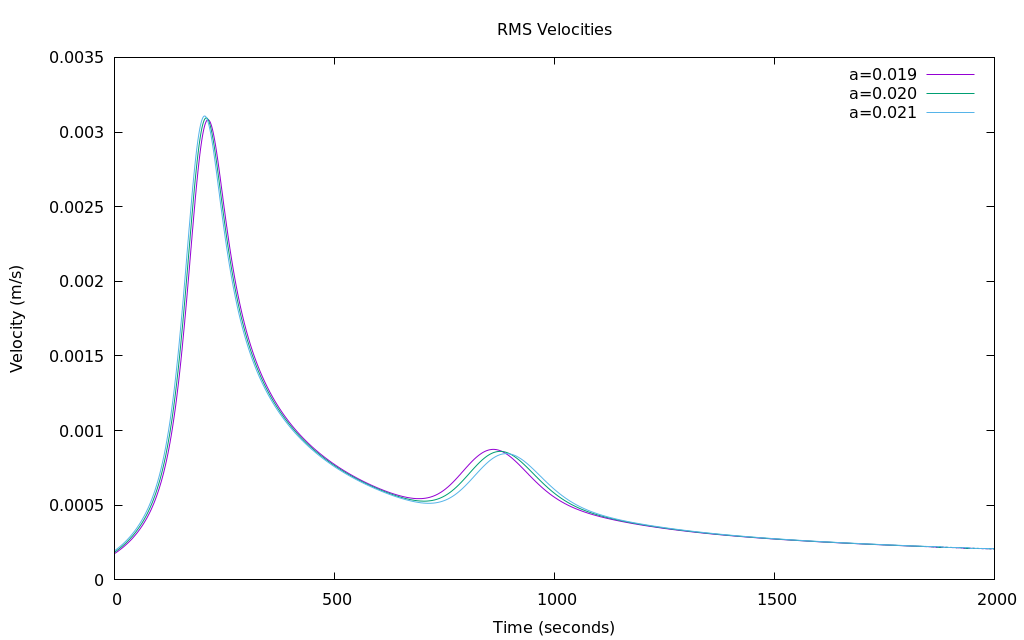
\includegraphics[width=0.5\textwidth]{cookbooks/van-keken-vof/doc/init_diff_rms_vel_comparison.png}
    \caption{\it Computations of the van Keken problem made with the VOF
        interface tracking algorithm showing the evolution of the RMS velocity
        as a function of time for small changes in the amplitude $a$ of the
        cosine function in the initial condition at 7 levels of refinement.
        Compare to Figures~\ref{fig:vk-6} and~\ref{fig:vof-vk-1}.
    }
    \label{fig:vof-vk-3}
\end{figure}

In these computations we vary the value of $a$ from its usual value of $a = 0.02$ to 
$5\% = 0.001$ below its usual value to $5\%$ above its usual value in increments of $0.01$.
In other words, we compare the values for $a =0.019$, $0.020$, and $0.021$.
Upon examination of Figure~\ref{fig:vof-vk-3}, we see a visible variation in the location of 
the second peak, although the overall shape of the curve remains consistent with the curves 
in Figure~\ref{fig:vof-vk-1}.
The size of this variation in the initial conditions cannot be expected to be reproduced using 
the standard compositional quadrature initialization procedure for VOF unless the cell size is on the scale 
of the change in the value of $a$; i.e., $h \, \lessapprox \, \Delta a = 0.001$.
We also note that the smoothing parameter which would produce a
$10^{-3}\leq C \leq 1 - 10^{-3}$ band on the order of the same size as the
amplitude variation shown here, would be approximately $2.8 \cdot 10^{-4}$.
This perturbation is much smaller than any of the changes in width of the smoothed regions in 
the computations shown in Figure~\ref{fig:vk-6}.
In summary, these results demonstrate the sensitivity of the discontinuous version of the van 
Keken problem to even extremely small variations in the initial conditions.
